\chapter{User Manual}\label{cap:evaluation}

\section{Requirements}
The application can be used in different area of application. The main requirement is to have a smartphone with a camera and a QR code reader. The application is available for Android and iOS. The application is available for free on the Google Play Store and the Apple App Store. The application is available in English and Romnian. The users will be able to import any model in the application using the QR code.

\section{Graphical overview of RealityEnhance}
We will now go through some of the application's graphical user interfaces. The following should summarise the fundamental flows present in the program and accommodate the user concerning the interface.
\pagebreak

\subsection{App start page}
The first thing any user will see when they launch the app on their phone is the loading page. This page is a simple loading screen displayed while the app is loading. In the loading phase, the app will check if the user can run the app on their phone and if the phone has the necessary sensors to run it. If the user can run the app, the app will load the main page. If the user cannot run the app, the app will display a message that the user cannot run the app on their phone.
\begin{figure}[h!]
    \begin{center}
        
\includegraphics[scale=0.5]{img/App_mock/iPhone 14 - 1.png}
        \caption{Loading page}
        \label{fig:loading-page}
    \end{center}
\end{figure}
\pagebreak


\subsection{App burger button}
The burger button is a button that is present on every page of the app. It is used to open the side menu. The side menu is used to navigate through the app. In the burger button, we can access the following options: QR scanner, Library, and EXIT.
The QR scanner scans a QR code and loads a 3D model and guide into the user's smartphone. The Library is used to display all the 3D models that the user has scanned. The EXIT button is used to exit the app.
\begin{figure}[h!]
    \begin{center}
        
\includegraphics[scale=0.5]{img/App_mock/iPhone 14 - 2.png}
        \caption{Burger button menu}
        \label{fig:burger-button}
    \end{center}
\end{figure}
\pagebreak

\subsection{QR scanner}
In this mode, a camera view will be displayed on the user's screen. The user will have to scan a QR code. The QR code will contain a link to a 3D model and a guide. The app will download the 3D model and the guide and display them on the user's screen. The model loaded from the QR code will be ready without entering the Library menu. The guide will be displayed on the user's screen, and the user must follow the guide to assemble the 3D model.

\begin{figure}[h!]
    \begin{center}
        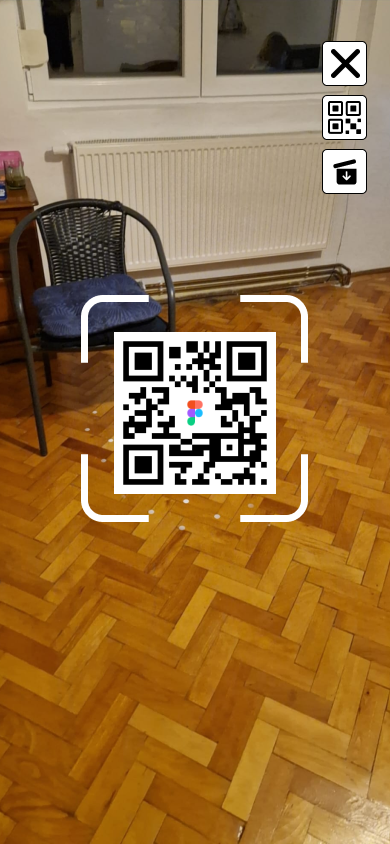
\includegraphics[scale=0.5]{img/App_mock/iPhone 14 - 3.png}
        \caption{QR scanner interface}
        \label{fig:qr-scanner}
    \end{center}
\end{figure}
\pagebreak

\subsection{QR valdiation}
If the QR code is valid, the app will display a message that the QR code is valid and will load the 3D model and the guide. If the QR code is not valid, the app will display a message that the QR code is not valid.

\begin{figure}[h!]
    \begin{center}
        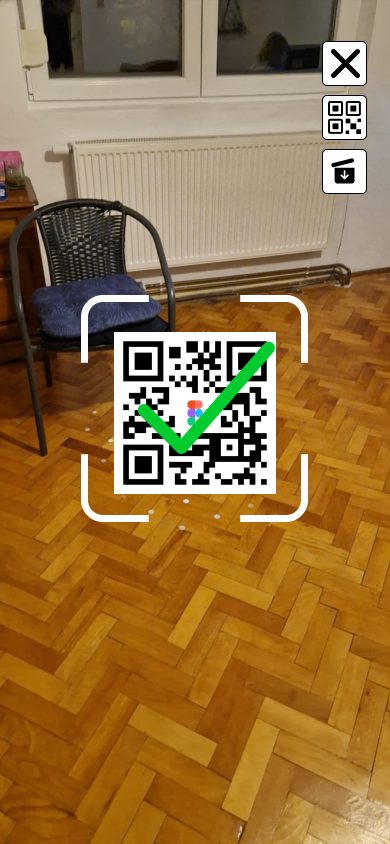
\includegraphics[scale=0.5]{img/App_mock/iPhone 14 - 4.png}
        \caption{QR code is valid}
        \label{fig:qr-valdiation}
    \end{center}
\end{figure}
\pagebreak

\subsection{AR vision}
After a model is loaded, the AR module will use the phone's camera to determine the user's surroundings. It will make a 3D model of the environment and place the 3D model on top of the environment. The user will have a guide of the app in understanding the surroundings (a mesh of the planes will be displayed on the screen).
\begin{figure}[h!]
    \begin{center}
        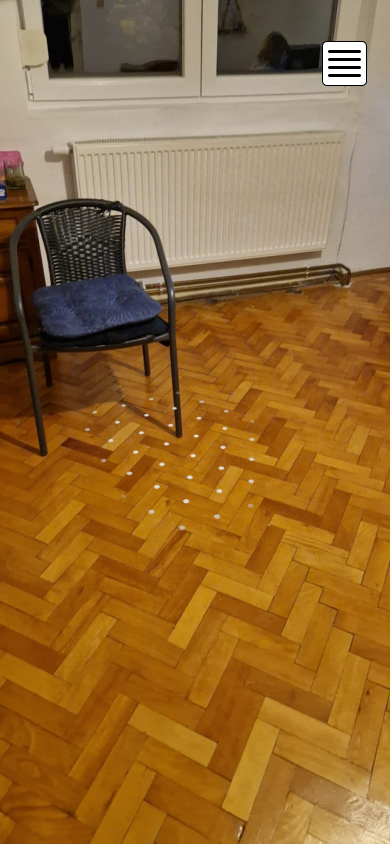
\includegraphics[scale=0.5]{img/App_mock/iPhone 14 - 5.png}
        \caption{AR vision interface}
        \label{fig:ar-vision}
    \end{center}
\end{figure}

\pagebreak

\subsection{Adding a model}
After the app has a basic understanding of the surroundings and a model loaded, the user can click on the screen to add an object to the scene. This object will be placed on the screen, and the user can move it around it. The user can move the object around the screen by press-and-hold the object and moving the phone around or dragging the object with his/her finger across the screen. The user will be able to rotate the object by rotating the model using two fingers (like opening a bottle cap(rotating clock-wised) or closing a bottle cap(rotating counter-clock-wised)). The user will be able to scale the object by pinching the screen. The user is not bound to use just a single object. The user can add multiple objects to the scene and move them around the screen. The user can add another object by clicking on the screen in a place where an object is not present.
\begin{figure}[!h]
    \begin{center}
        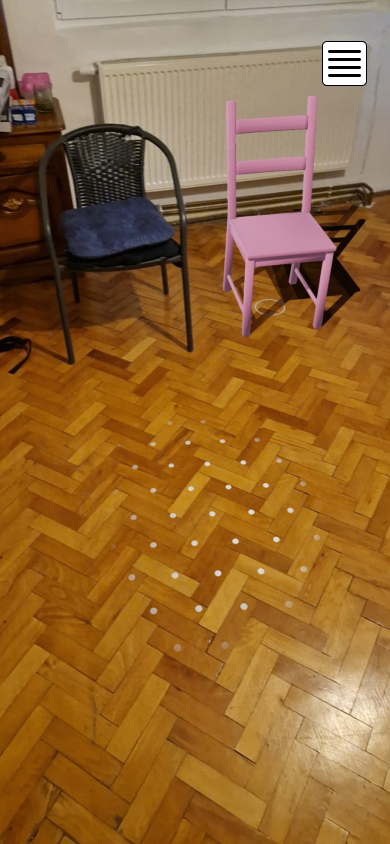
\includegraphics[scale=0.5]{img/App_mock/iPhone 14 - 6.png}
        \caption{Adding a model}
        \label{fig:add-a-model}
    \end{center}
\end{figure}
\pagebreak

\subsection{Removing a model}
The user can remove the object by clicking and holding on the object and then clicking on the remove button. The user will be able to remove multiple objects at the same time by clicking on the reset all button.
\begin{figure}[h!]
    \begin{center}
        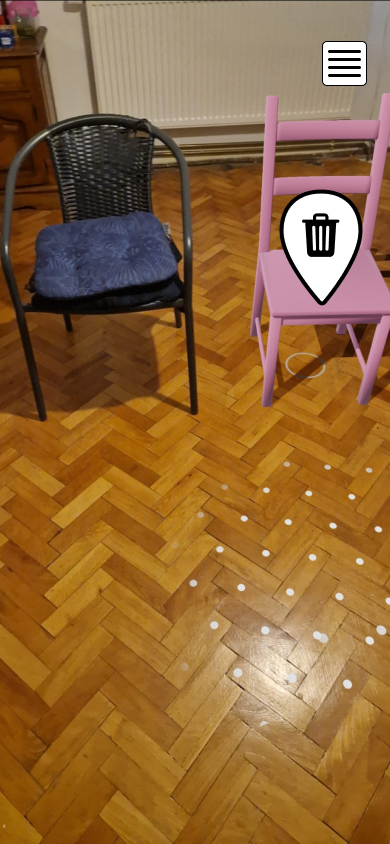
\includegraphics[scale=0.5]{img/App_mock/iPhone 14 - 7.png}
        \caption{Removing a model}
        \label{fig:remove-a-model}
    \end{center}
\end{figure}
\pagebreak


\begin{center}
    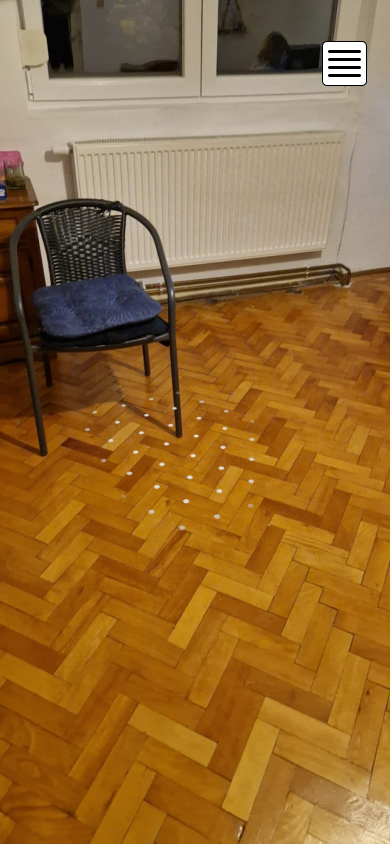
\includegraphics[scale=0.5]{img/App_mock/iPhone 14 - 8.png}
\end{center}
\pagebreak

\begin{center}
    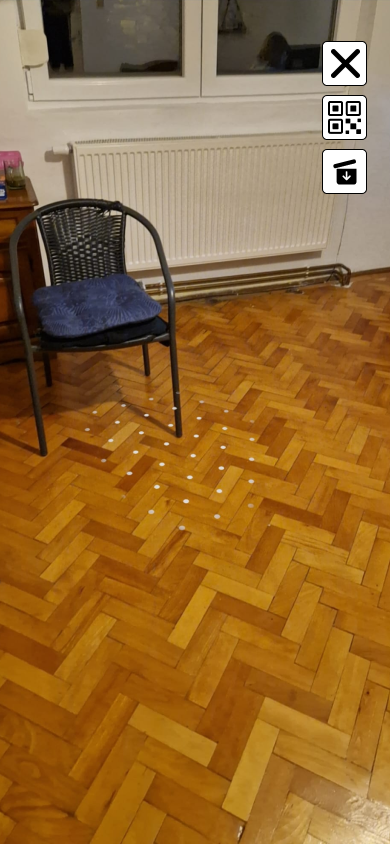
\includegraphics[scale=0.5]{img/App_mock/iPhone 14 - 9.png}
\end{center}
\pagebreak

\subsection{Library}
The app will display the Library interface when the user clicks on the Library button in the burger menu. The Library interface will display all the 3D models the user has scanned. The user can select a model and load it into the AR vision mode. In the Library interface, the user can search for and add a model to the Library. The user can also delete a model from the Library.
\begin{figure}[h!]
    \begin{center}
        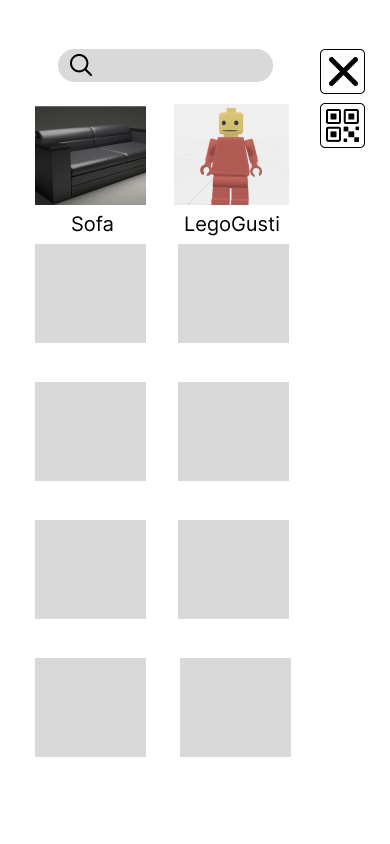
\includegraphics[scale=0.5]{img/App_mock/iPhone 14 - 10.png}
        \caption{Library interface}
        \label{fig:library}
    \end{center}
\end{figure}
\pagebreak

\subsection{Using multiple models at the same time}
The user will be able to use multiple models at the same time. The user can add multiple models to the scene and move them around the screen. The user can add another model by clicking on the screen in a place where an object is not present. The guide for assembling or building a model will be displayed on the screen when the scene has just one object.
\begin{figure}[h!]
    \begin{center}
        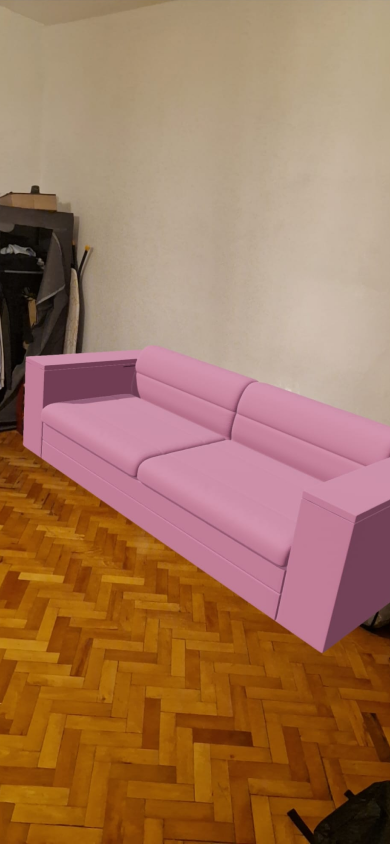
\includegraphics[scale=0.5]{img/App_mock/iPhone 14 - 11.png}
        \caption{Using multiple models}
        \label{fig:using-multiple-models}
    \end{center}
\end{figure}
\pagebreak
